\documentclass[xcolor=dvipsnames]{beamer}
\usepackage{calligra}
\usepackage{amsmath}
\usepackage{amsthm}
\usepackage{mathrsfs}
\usepackage{graphicx}
\usepackage{bm}
\usepackage{multimedia}
\usepackage{colortbl}

\usefonttheme{serif}
\usecolortheme[named=BrickRed]{structure}
\usetheme[height=7mm]{Rochester}
%\usetheme{default}
\title{\small{Generally Covariant Hamiltonian Approach\\to\\Generalized Harmonic Formulation of General Relativity}}
\author[M. Cao]{Meng Cao\\Advisor: Dr. John David Brown}
\institute[NCSU]{Department of Physics\\North Carolina State University\\Raleigh, NC 27695\\
\texttt{mcao2@ncsu.edu}}
\date[March 2014]{March 2014}
\begin{document}
	\begin{frame}
		\titlepage
	\end{frame}
	\begin{frame}{Outline}
		\begin{itemize}
			\item{Introduction}
			\item{Numerical Relativity}
			\item{General Covariance}
			\item{Hamiltonian Approach}
			\item{Summary and Future Work}
		\end{itemize}
	\end{frame}
	\begin{frame}{Introduction}
		\begin{itemize}
			\item{General Relativity}
			\item{Hamiltonian Formulation}
			%\item{Notation and Convention}
		\end{itemize}
	\end{frame}
	\begin{frame}{Introduction}
		General Relativity
		\begin{columns}[c]
			\column{2in}
			\begin{center}
				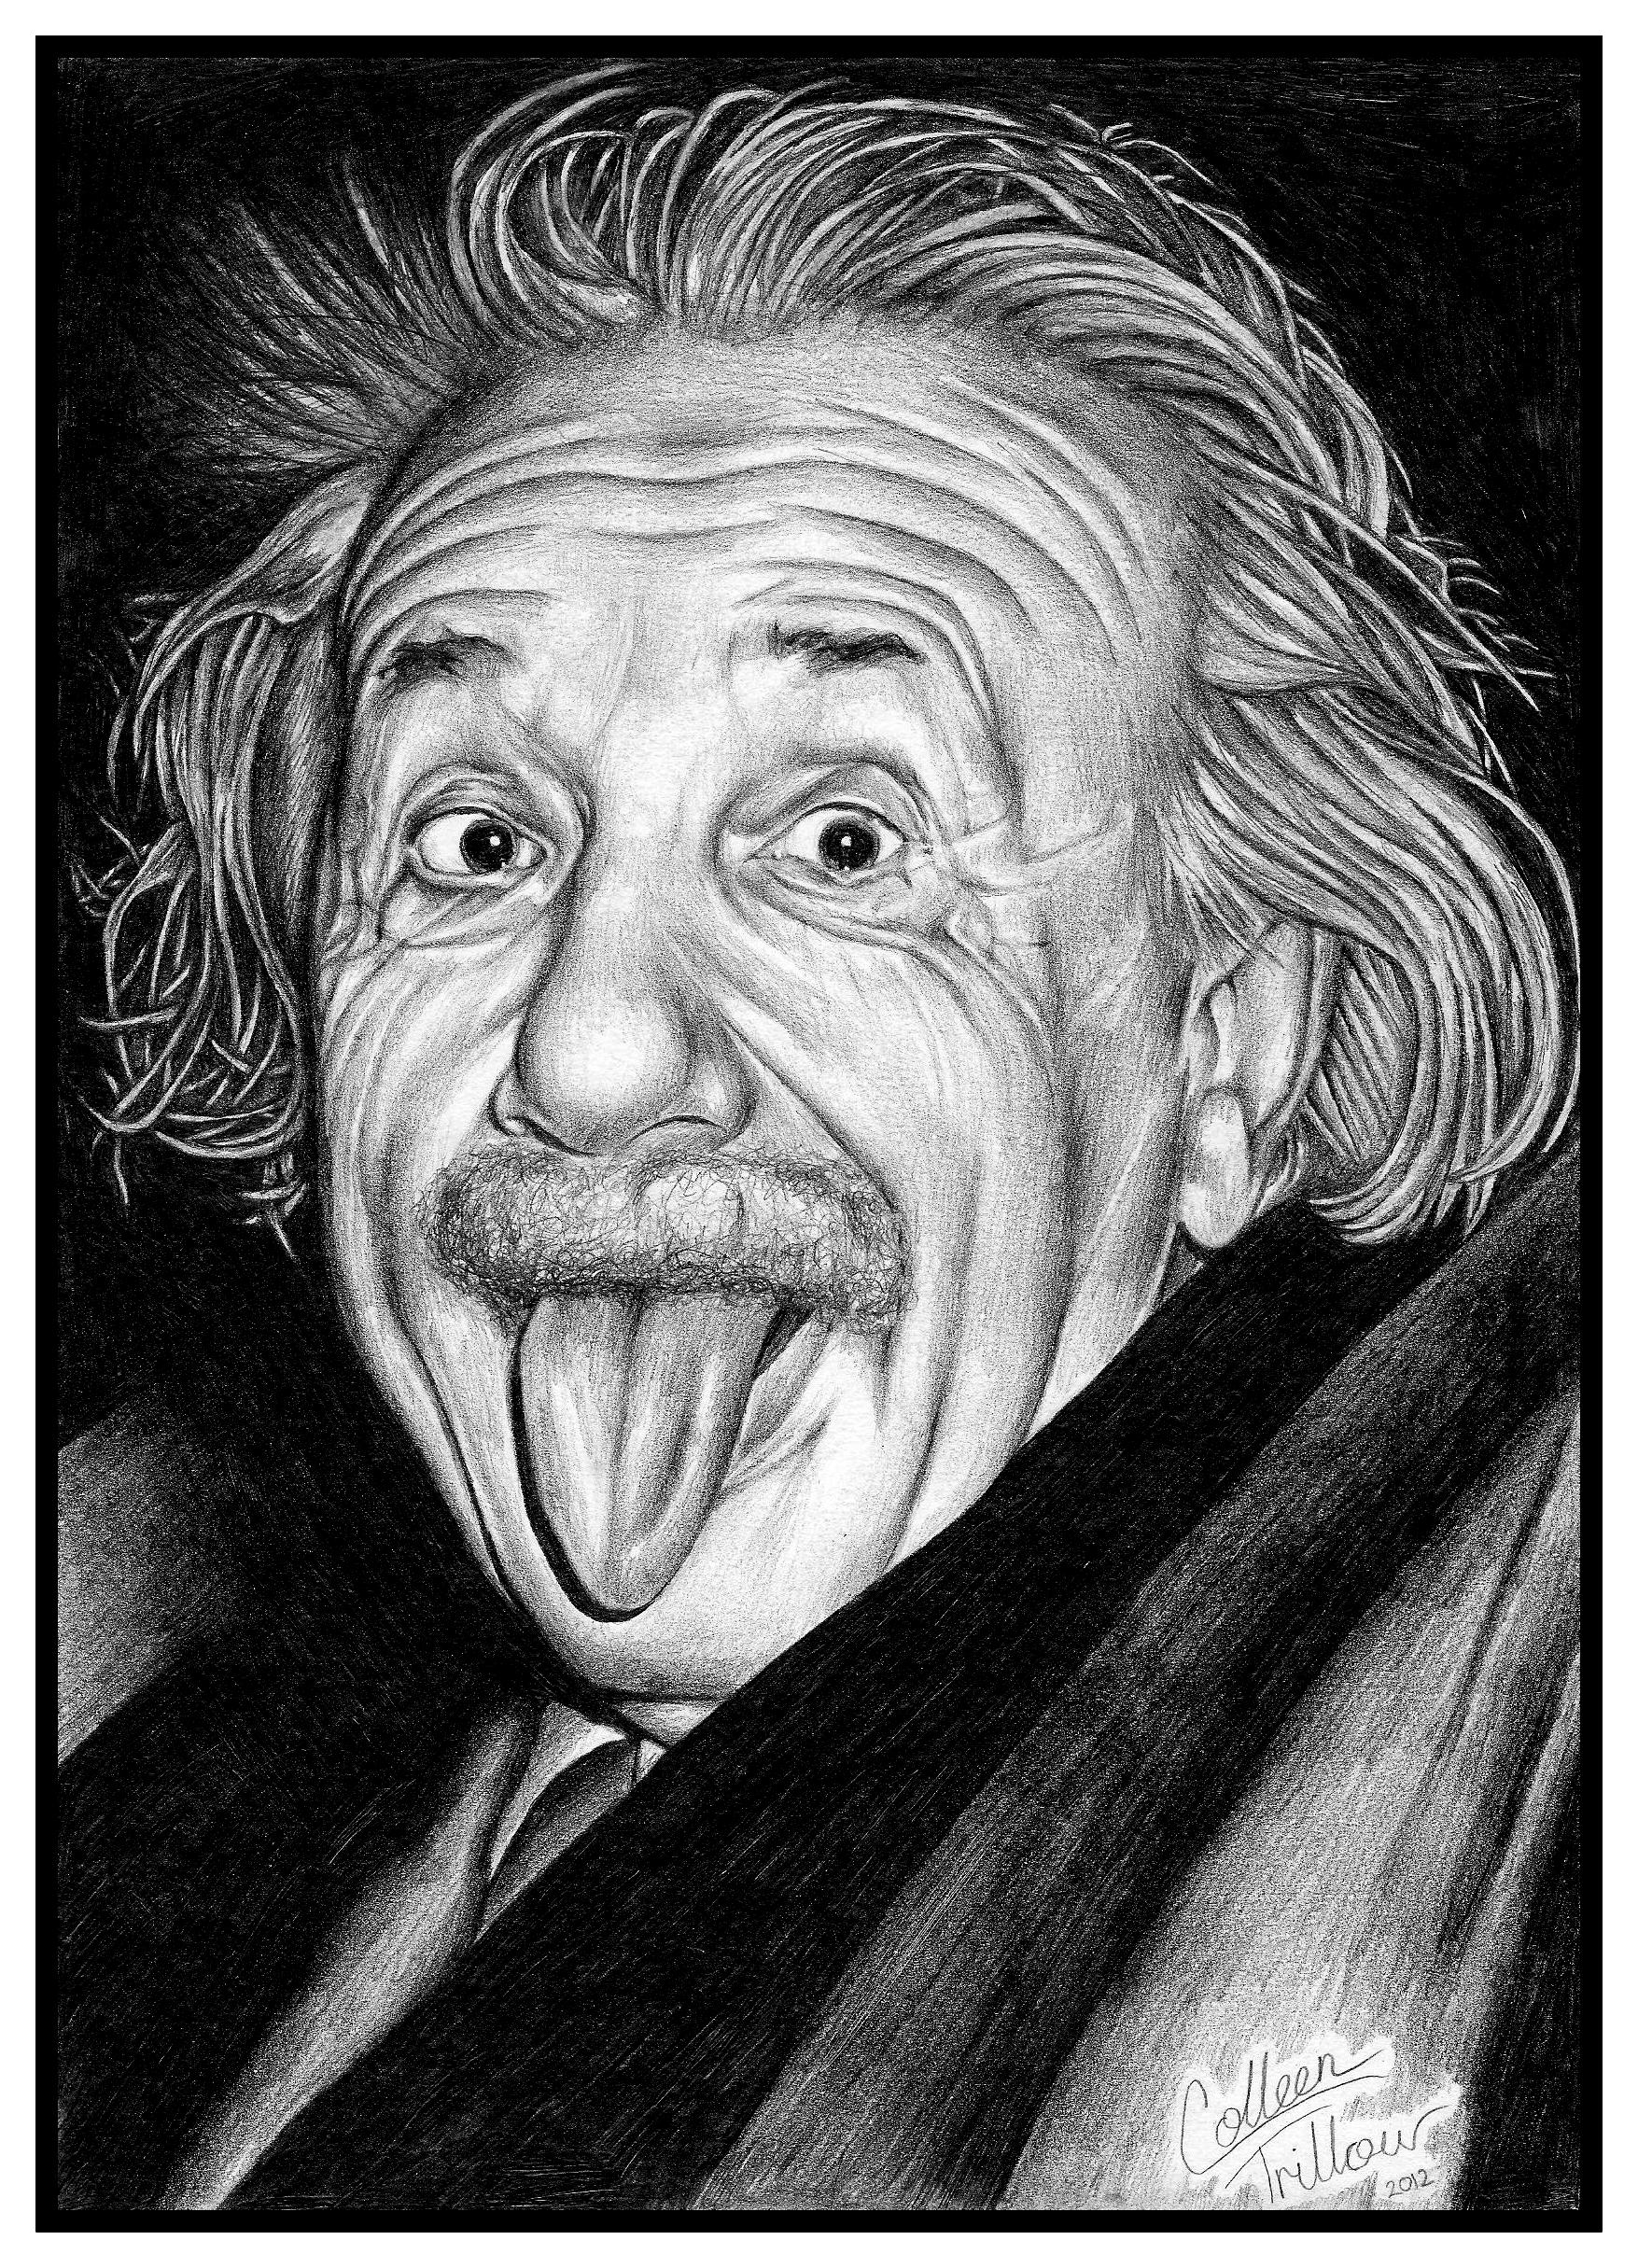
\includegraphics[scale=0.07]{einstein.jpg}\\
				\tiny{Colleen Trillow}
			\end{center}
			\column{2in}
			\begin{center}
				\includegraphics[scale=0.23]{grpaper.pdf}
			\end{center}
		\end{columns}
	\end{frame}
	\begin{frame}{Introduction}
		General Relativity
		\begin{center}
			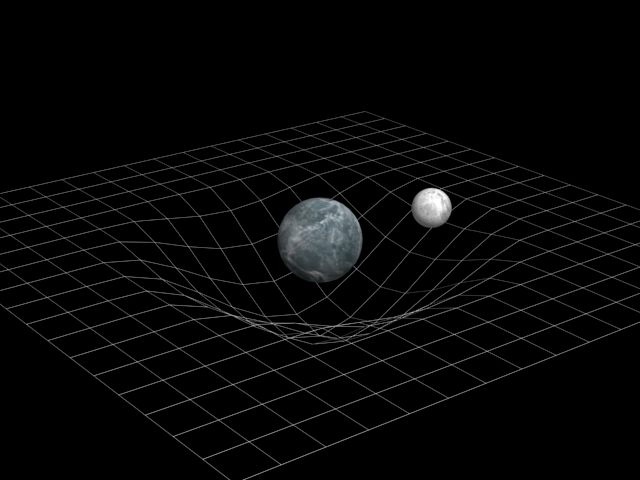
\includegraphics[scale=0.4]{curvature.jpg}
		\end{center}
	\end{frame}
	\begin{frame}{Introduction}
		Classical Tests of General Relativity
		\begin{itemize}
			\item{Light Deflection[Eddington, 1919]}
			\item{Perihelion Precession of Mercury[Urbain Le Verrier, 1859]}
			\item{Gravitational Redshift[Pound-Rebka, 1959]}
		\end{itemize}
	\end{frame}
	\begin{frame}{Introduction}
		Breakthrough on March 17th, 2014
		\pause
		\begin{center}
			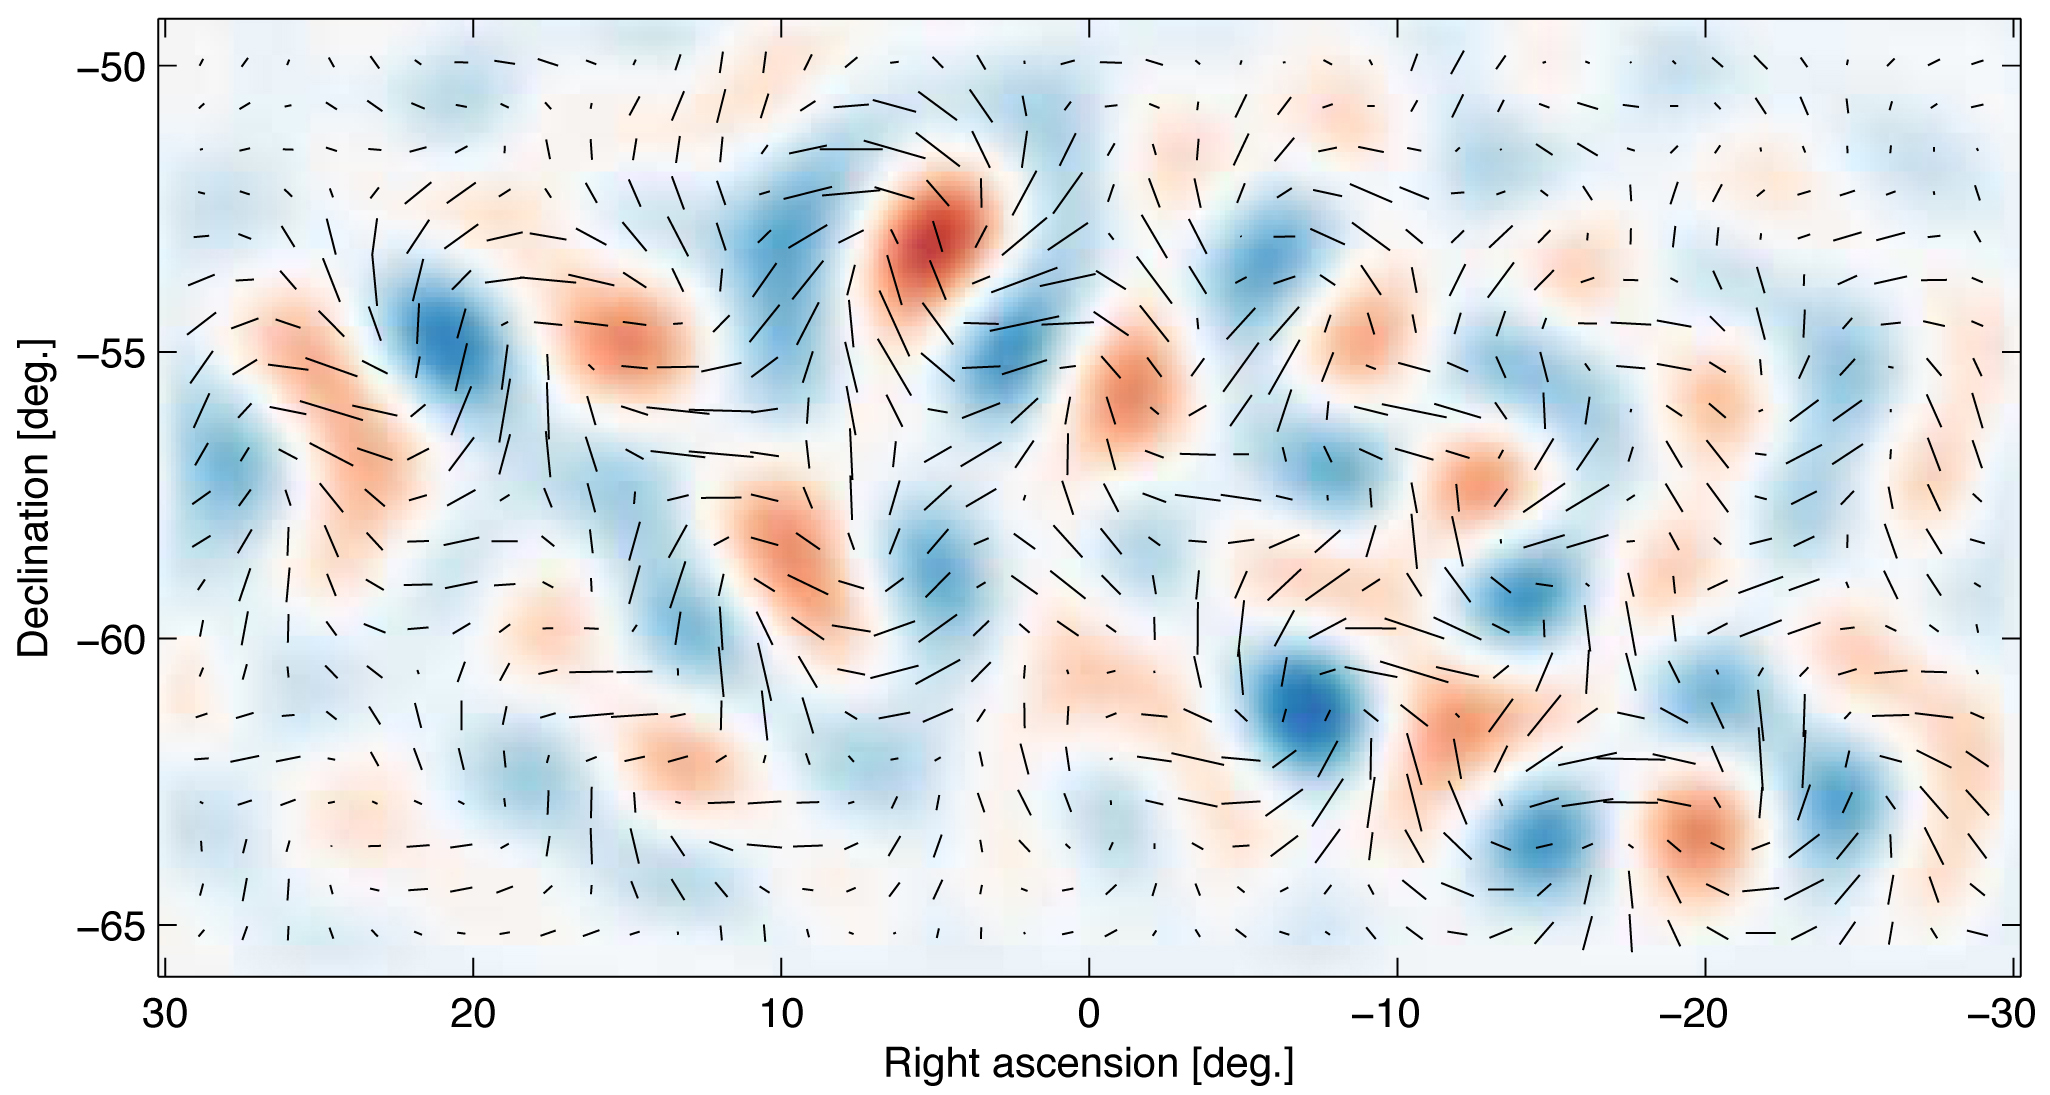
\includegraphics[scale=0.6]{bicep2-hires.jpg}\\
			\tiny{BICEP2 Collaboration}
		\end{center}
	\end{frame}
	\begin{frame}{Introduction}
		Breakthrough on March 17th, 2014
		\begin{center}
			\includegraphics[scale=0.3]{bicep2.jpg}\\
			\tiny{Steffen Richter (Harvard University)}
		\end{center}
	\end{frame}
	\begin{frame}{Introduction}
		Einstein Field Equations
		\huge
		\begin{center}
			\[
			G_{\mu\nu} = 8\pi T_{\mu\nu}
			\]
		\end{center}
	\end{frame}
	\begin{frame}{Introduction}
		Exact Solutions to Einstein Field Equations
		\begin{center}
			\Large
			\begin{tabular}{|c c c|}
				\hline
				\cellcolor[gray]{0.7}~ & \cellcolor[gray]{0.9}$J=0$ & $J \ne 0$ \\
				\rowcolor[gray]{0.9}$Q=0$ & \cellcolor[gray]{1.0}Schwarzschild & \cellcolor[gray]{0.7}Kerr \\
				\cellcolor[gray]{1.0}$Q\ne 0$ & \cellcolor[gray]{0.7}Reissner-Nordstr\"{o}m & \cellcolor[gray]{0.9}Kerr-Newman\\ \hline
			\end{tabular}
		\end{center}
	\end{frame}
	\begin{frame}{Introduction}
		Numerical Relativity
		\begin{columns}[c]
			\column{2in}
			\begin{center}
				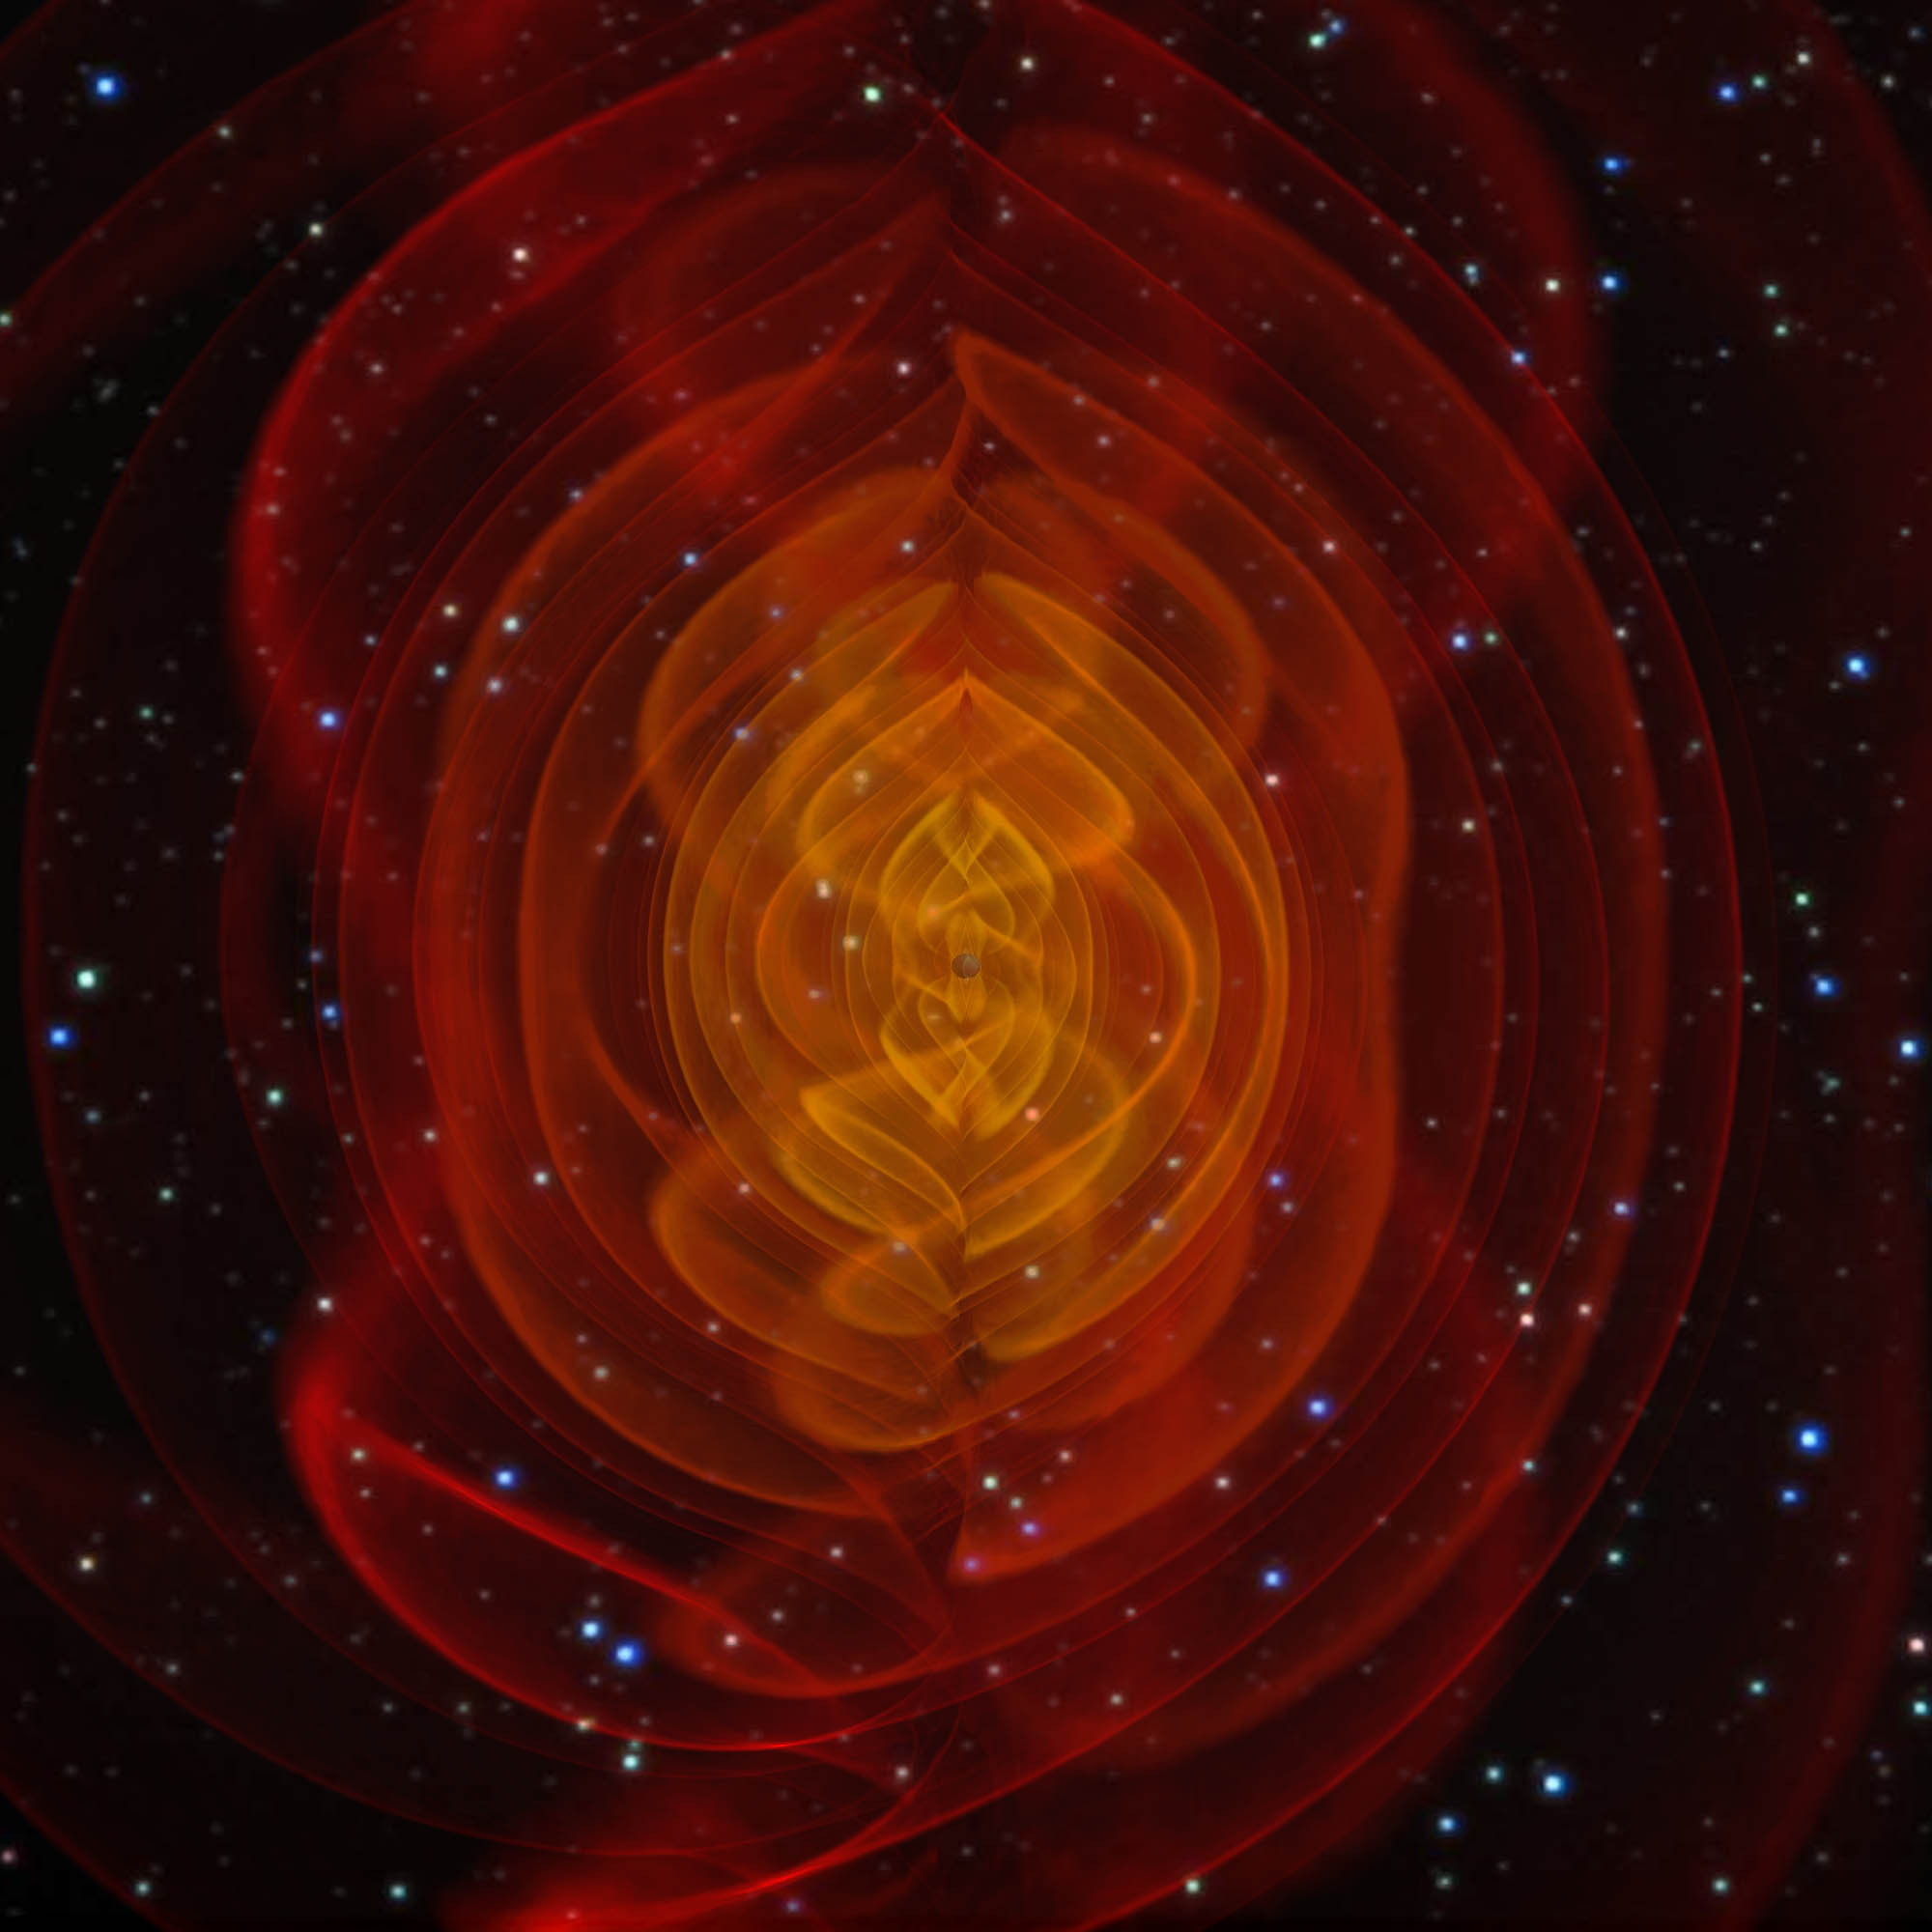
\includegraphics[scale=0.07]{nr-baker.jpg}\\
				\tiny{simulation: John Baker (NASA)}\\
				\tiny{visualization: Henze (NASA)}
			\end{center}
			\column{2in}
			\begin{center}
				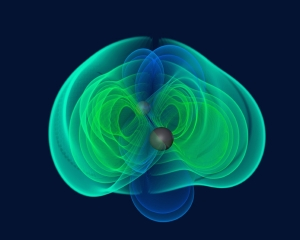
\includegraphics[scale=0.5]{nr-mpg.jpg}\\
				\tiny{simulation: C. Reisswig, L. Rezzolla (Albert Einstein Institute)}\\
				\tiny{visualization: M. Koppitz (Albert Einstein Institute/Zuse Institute Berlin)}
			\end{center}
		\end{columns}		
	\end{frame}
	\begin{frame}{Introduction}
		Hamiltonian Formulation
		\begin{center}
			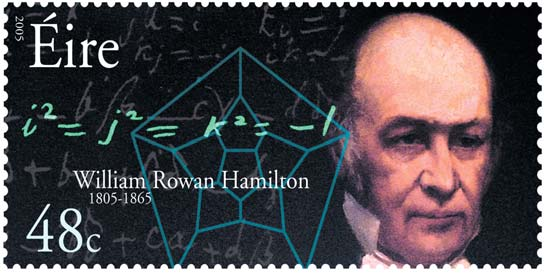
\includegraphics[scale=1.0]{hamilton.jpg}\\
			\tiny{Sir William Rown Hamilton(1805 - 1865)}
		\end{center}
	\end{frame}
	\begin{frame}{Introduction}
		Lagrangian vs Hamiltonian
		\begin{columns}[c]
			\column{2in}
			\begin{center}
				$\mathcal{L}(q_{i}, {\dot q}_{i}, t)$
				\begin{equation*}
					\frac{\partial}{\partial t}\frac{\partial \mathcal{L}}{\partial {\dot q_{i}}} - \frac{\partial \mathcal{L}}{\partial q_{i}} = 0
				\end{equation*}	
			\end{center}
			\column{2in}
			\begin{center}
				$\mathcal{H}(q_{i}, p_{i}, t)$	
				\begin{align*}
					{\dot p}_{i} + \frac{\partial \mathcal{H}}{\partial q_{i}} &= 0	\\
					{\dot q}_{i} - \frac{\partial \mathcal{H}}{\partial p_{i}} &= 0
				\end{align*}
			\end{center}
		\end{columns}
		\pause
		\begin{center}
			\Large{mathematically equivalent}
		\end{center}
	\end{frame}
	\begin{frame}{Introduction}
		Advantages of Hamiltonian Formulation
		\begin{itemize}
			\item{Equal status of coordinates and momenta}
			\item{More abstract presentation of physics}
			\item{Embarking point of modern theories}
		\end{itemize}
	\end{frame}
	\begin{frame}{Numerical Relativity}
		\textbf{\textit{"If a corresponding large class of solutions of Einstein’s equation failed to exist, we would be forced to reject general relativity as a correct theory of nature"}}\\
		\hfill \textbf{--- Wald}
	\end{frame}
	\begin{frame}{Numerical Relativity}
		\begin{itemize}
			\item{3 + 1 Decomposition}
			\item{Numerical Formulations}
		\end{itemize}
	\end{frame}
	\begin{frame}{Numerical Relativity}
		3 + 1 Decomposition
		\begin{center}
			\Huge{\textbf{\textit{Demo}}}
		\end{center}
	\end{frame}
	\begin{frame}{Numerical Relativity}
		3 + 1 Decomposition
		\Large
		\[
		ds^{2} = - \alpha^{2}dt^{2} + g_{ab}(dx^{a} + \beta^{a}dt)(dx^{b} + \beta^{b}dt) 		
		\]
	\end{frame}
	\begin{frame}{Numerical Relativity}
		3 + 1 Decomposition
		\begin{center}
			\Large
			$g_{ab}~~~~\alpha~~~~\beta^{a}~~~~K_{ab}$
		\end{center}
	\end{frame}
	\begin{frame}{Numerical Relativity}
		Numerical Formulations
		\begin{itemize}
			\pause
			\item{ADM/BSSN}
			\pause
			\begin{itemize}
				\item{Arnowitt, Deser and Misner}
			\pause
				\item{Baumgarte, Shapiro, Shibata and Nakamura}
			\end{itemize}
			\pause
			\item{Generalized Harmonic}
			\pause
			\begin{itemize}
				\item{Friedrich, 1985; Garfinkle, 2002; Pretorius, 2006}
			\end{itemize}
		\end{itemize}
	\end{frame}
	\begin{frame}{Numerical Relativity}
		Motivation
		\begin{itemize}
			\item{Importance of Hamiltonian formalism}
			\item{Well-posedness of GH formualation}
			\pause
			\item{3 + 1 form of GH equations[Brown, 2011]}
			\item{Action principle for GH formulation[Brown, 2011]}
		\end{itemize}
	\end{frame}
	\begin{frame}{General Covariance}
		General Covariance
		\pause
		\Large
		\[
		G_{\mu\nu} = 8\pi T_{\mu\nu}
		\]
		\pause
		\[
		x^{\mu} \rightarrow x^{\mu'}
		\]
		\pause
		\[
		G_{\mu'\nu'}\frac{\partial x^{\mu'}}{\partial x^{\mu}}\frac{\partial x^{\nu'}}{\partial x^{\nu}} = 8 \pi T_{\mu'\nu'}\frac{\partial x^{\mu'}}{\partial x^{\mu}}\frac{\partial x^{\nu'}}{\partial x^{\nu}}
		\]
	\end{frame}
	\begin{frame}{General Covariance}
		3 + 1 Coordinate Transformation
		\begin{itemize}
			\item{General class}
			\item{Preserve 3 + 1 structure}
		\end{itemize}
	\end{frame}
	\begin{frame}{General Covariance}
		Foliation Preserving Transformation
		\pause
		\begin{align*}
		t' &= t'(t)\text{  : time reparameterization}\\
		x^{a'} &= x^{a'}(t, x^{a})\text{  : time-dependent spatial transformation}
	\end{align*}
	\end{frame}
	\begin{frame}{General Covariance}
		Tensorial Transformation
		\[
		T^{a_{1}'...a_{n}'}_{~~~~~~~~b_{1}'...b_{m}'} = T^{a_{1}...a_{n}}_{~~~~~~~~b_{1}...b_{n}}\frac{\partial x^{a_{1}'}}{\partial x^{a_{1}}}...\frac{\partial x^{a_{n}'}}{\partial x^{a_{n}}}\frac{\partial x^{b_{1}}}{\partial x^{b_{1'}}}...\frac{\partial x^{b_{m}}}{\partial x^{b_{m'}}}\left|\frac{\partial t}{\partial t'}\right|^{i}\left|\frac{\partial x}{\partial x'}\right|^{j} 
		\]
		\pause
		\begin{itemize}
			\item{weight i tensor density under time reparameterization}
			\item{type $n\choose m$ weight j tensor density under time-dependent spatial transformation}
		\end{itemize}
	\end{frame}
	\begin{frame}{General Covariance}
		Transformation Rules
		\begin{align*}
		g_{a'b'} & = g_{ab}\frac{\partial x^{a}}{\partial x^{a'}}\frac{\partial x^{b}}{\partial x^{b'}}\\
		g^{a'b'} & = g^{ab}\frac{\partial x^{a'}}{\partial x^{a}}\frac{\partial x^{b'}}{\partial x^{b}}\\
		g' & = g\left|\frac{\partial x}{\partial x'}\right|^{2}
	\end{align*}
	\end{frame}
	\begin{frame}{General Covariance}
		Transformation Rules
			\[
				\alpha' = \alpha \frac{\partial t}{\partial t'}
			\]
			\pause
			\begin{align*}
				\beta^{a'} &= \beta^{a}\frac{\partial x^{a'}}{\partial x^{a}}\frac{\partial t}{\partial t'} + \frac{\partial x^{a'}}{\partial x^{a}}\frac{\partial x^{a}}{\partial t'}\\
				\beta_{a'} &= \beta_{a}\frac{\partial x^{a}}{\partial x^{a'}}\frac{\partial t}{\partial t'} + g_{ab}\frac{\partial x^{a}}{\partial x^{a'}}\frac{\partial x^{b}}{\partial t'}				
			\end{align*}
	\end{frame}
	\begin{frame}{General Covariance}
		Background Metric
		\pause
		\begin{align*}
		{\bar g}_{ab} &= \text{diag}(1, 1, 1)\\
		{\bar \alpha} &= 1\\
		{\bar \beta}^{a} &= (0, 0, 0)
		\end{align*}
	\end{frame}
	\begin{frame}{General Covariance}
		Transformation Rules
		\[
		\beta^{a'} = \beta^{a}\frac{\partial x^{a'}}{\partial x^{a}}\frac{\partial t}{\partial t'} + \frac{\partial x^{a'}}{\partial x^{a}}\frac{\partial x^{a}}{\partial t'}
		\]
		\pause
		\[
		{\bar \beta}^{a'} = {\bar \beta}^{a}\frac{\partial x^{a'}}{\partial x^{a}}\frac{\partial t}{\partial t'} + \frac{\partial x^{a'}}{\partial x^{a}}\frac{\partial x^{a}}{\partial t'}
		\]
		\pause
		\[
		\Delta \beta^{a} \equiv \beta^{a} - {\bar \beta}^{a}
		\]
		\pause
		\[
		\Delta \beta^{a'} = \Delta\beta^{a}\frac{\partial x^{a'}}{\partial x^{a}}\frac{\partial t}{\partial t'}
		\]
	\end{frame}
	\begin{frame}{General Covariance}
		Transformation Rules
		\begin{align*}
			D_{c'}g_{a'b'} &= D_{c}g_{ab}\frac{\partial x^{c'}}{\partial x^{c}}\frac{\partial x^{a'}}{\partial x^{a}}\frac{\partial x^{b'}}{\partial x^{b}}\\
		D_{a'}\alpha' &= D_{a}\alpha\frac{\partial x^{a}}{\partial x^{a'}}\frac{\partial t}{\partial t'}\\
		D_{a'}\Delta\beta^{b'} &= D_{a}\Delta\beta^{b}\frac{\partial x^{a}}{\partial x^{a'}}\frac{\partial x^{b'}}{\partial x^{b}}\frac{\partial t}{\partial t'}	
		\end{align*}
	\end{frame}
	\begin{frame}{General Covariance}
		Transformation Rules
		\begin{align*}
			\partial_{t'}g_{a'b'} &=  \left(\partial_{t}g_{ab}\right)\frac{\partial t}{\partial t'}\frac{\partial x^{a}}{\partial x^{a'}}\frac{\partial x^{b}}{\partial x^{b'}} + \left(\partial_{c}g_{ab}\right)\frac{\partial x^{c}}{\partial t'}\frac{\partial x^{a}}{\partial x^{a'}}\frac{\partial x^{b}}{\partial x^{b'}} \\
			&+ g_{ab}\partial_{t'}\left(\frac{\partial x^{a}}{\partial x^{a'}}\frac{\partial x^{b}}{\partial x^{b'}}\right)\\
			\partial_{t'}\alpha' &= \partial_{t}\alpha\left(\frac{\partial t}{\partial t'}\right)^{2} + \partial_{c}\alpha\frac{\partial x^{c}}{\partial t'}\frac{\partial t}{\partial t'} + \alpha\frac{\partial^{2}t}{\partial {t'}^{2}}\\
			\partial_{t'}\Delta \beta^{a'} &= \partial_{t}\Delta \beta^{a}\frac{\partial x^{a'}}{\partial x^{a}}\left(\frac{\partial t}{\partial t'}\right)^{2} + \partial_{c}\Delta \beta^{a}\frac{\partial x^{c}}{\partial t'}\frac{\partial x^{a'}}{\partial x^{a}}\frac{\partial t}{\partial t'}\notag\\
			& + \Delta \beta^{a}\frac{\partial x^{a'}}{\partial x^{a}}\frac{\partial^{2}t}{\partial t'^{2}} + \Delta \beta^{a}\frac{\partial^{2} x^{a'}}{\partial x^{c}\partial x^{a}}\frac{\partial x^{c}}{\partial t'}\frac{\partial t}{\partial t'} + \Delta \beta^{a}\frac{\partial^{2}x^{a'}}{\partial t\partial x^{a}}\left(\frac{\partial t}{\partial t'}\right)^{2}
		\end{align*}
	\end{frame}
	\begin{frame}{General Covariance}
		Covariant Time Derivative
		\[
			D_{t}g_{ab} \equiv (\partial_{t} - \mathcal{L}_{\beta})g_{ab} = -2\alpha K_{ab}
		\]
		\pause
		any scalar under time reparameterization
		\[
			D_{t} \equiv \partial_{t} - \mathcal{L}_{\beta} 
		\]		
	\end{frame}
	\begin{frame}{General Covariance}
		Covariant Time Derivative
		\[
		D_{t}\alpha \equiv \partial_{t}\alpha - \beta^{c}\partial_{c}\alpha - \frac{\alpha}{{\bar \alpha}}\left(\partial_{t}{\bar \alpha} - {\bar \beta}^{c}\partial_{c}{\bar \alpha}\right)
		\]
		\pause
		\[
		D_{t}\beta^{a} \equiv \partial_{t}\Delta \beta^{a} - \frac{\Delta \beta^{a}}{{\bar \alpha}}\left(\partial_{t}{\bar \alpha} - {\bar \beta}^{b}\partial_{b}{\bar \alpha}\right) - \beta^{b}{\bar D}_{b}\Delta \beta^{a} + \Delta \beta^{b}{\bar D}_{b}{\bar \beta}^{a}
		\]
	\end{frame}
	\begin{frame}{General Covariance}
		Gauge Conditions
		\pause
		\begin{align*}
			\partial_{t}\alpha - \beta^{c}\partial_{c}\alpha &= -2\alpha K\\
			\partial_{t}\beta^{a} - \beta^{b}\partial_{b}\beta^{a} &=  \frac{3}{4}{\tilde \Gamma}^{a} - \eta \beta^{a}
		\end{align*}
		\tiny
		\[
		\left[{\tilde \Gamma}^{a} \equiv \sqrt{g}^{2/3}\left(\Gamma^{a}_{~bc}g^{bc} + \frac{1}{3}g^{ab}\Gamma^{c}_{~bc}\right)\right]
		\]
	\end{frame}
	\begin{frame}{General Covariance}
		Covariant Gauge Conditions
		\pause
		\begin{itemize}
			\item{Replace non-tensorial terms with tensorial terms}
			\item{Balance density weights on both sides of equation}
		\end{itemize}
	\end{frame}
	\begin{frame}{General Covariance}
		Covariant Gauge Conditions
		\begin{align*}
			D_{t}\alpha &= -2\alpha{\bar \alpha}K\\
			D_{t}\beta^{a} &= \frac{3}{4}{\bar \alpha}^{2}\Delta {\tilde \Gamma}^{a} - \eta {\bar \alpha}\Delta\beta^{a}  
		\end{align*}
		\tiny
		\[
			\left[\Delta {\tilde \Gamma}^{a} \equiv \sqrt{\frac{g}{{\bar g}}}^{2/3}\left(\Delta \Gamma^{a}_{~bc}g^{bc} + \frac{1}{3}g^{ab}\Delta \Gamma^{c}_{~bc}\right)\right]
		\]
	\end{frame}
	\begin{frame}{Hamiltonian Approach}
		\begin{itemize}
			\item{Einstein-Hilbert Action}
			\item{Non-covariant Hamiltonian System}
			\item{Covariant Hamiltonian System}
			\item{Well-posedness}
		\end{itemize}
	\end{frame}
	\begin{frame}{Hamiltonian Approach}
		Einstein-Hilbert Action
		\begin{align*}
			\begin{split}
				&S\left[g_{ab}, \alpha, \beta^{a}, H_{\perp}, H^{a}\right] =\\&\int d^{4}x~~\alpha \sqrt{g} \left( R + K^{ab}K_{ab} - K^{2} - \frac{1}{2}C^{a}C_{a} + \frac{1}{2}C_{\perp}^{2}\right)
			\end{split}
		\end{align*}
		\tiny
		\[		
		\left[ C_{\perp} = H_{\perp} + K + \frac{1}{\alpha^{2}}D_{t}\alpha, C_{a} = H_{a} + \Delta \Gamma^{b}_{cd}g^{cd}g_{ab} - \frac{\partial_{a}\alpha}{\alpha} - \frac{g_{ab}}{\alpha^2}D_{t}\beta^{b} \right]
		\]
		\pause
		\normalsize
		\[
		S = \int\mathscr{L}d^{4}x
		\]
	\end{frame}
	\begin{frame}{Hamiltonian Approach}
		Conjugate Momenta
		\[
		p = \frac{\partial \mathscr{L}}{\partial {\dot q}}
		\]
		\pause
		\begin{align*}
			P^{ab} & \equiv \frac{\partial \mathscr{L}}{\partial {\dot g}_{ab}} = \sqrt{g}\left(Kg^{ab} - K^{ab} - \frac{C_{\perp}}{2}g^{ab}\right)\\
				\pi & \equiv \frac{\partial \mathscr{L}}{\partial {\dot \alpha}} = \frac{\sqrt{g}}{\alpha}C_{\perp}\\
				\rho_{a} & \equiv \frac{\partial \mathscr{L}}{\partial {\dot \beta}^{a}} = \frac{\sqrt{g}}{\alpha}C_{a}\\
				\Omega & \equiv \frac{\partial \mathscr{L}}{\partial {\dot H}_{\perp}} = 0\\
				\Omega_{a} & \equiv \frac{\partial \mathscr{L}}{\partial {\dot H}^{a}} = 0	
		\end{align*}
	\end{frame}
	\begin{frame}{Hamiltonian Approach}
		Hamiltonian
		\[
		\mathscr{H} \equiv P^{ab}{\dot g}_{ab} + \pi{\dot \alpha} + \rho_{a}{\dot \beta}^{a} + \Omega {\dot H}_{\perp} + \Omega_{a}{\dot H}^{a} - \mathscr{L}
		\]
	\end{frame}
	\begin{frame}{Hamiltonian Approach}
		Constraint Multiplier
		\begin{align*}
		{\dot H}_{\perp} & = \Lambda\\
		{\dot H}^{a} & = \Lambda^{a}
	\end{align*}
	\end{frame}
	\begin{frame}{Hamiltonian Approach}
		Hamiltonian
		\begin{align*}
			\mathscr{H} &= \frac{\alpha}{\sqrt{g}}\left(P^{ab}P_{ab} - \frac{P^{2}}{2} - \frac{\alpha P \pi}{2} + \frac{\alpha^{2}\pi^{2}}{8} - \frac{\alpha^{2}}{2}\rho_{a}\rho^{a}\right)\\
			& -\alpha^{2}\pi H_{\perp} + \alpha^{2}\rho_{a}H^{a} + \alpha^{2}\Delta\Gamma^{a}_{~bc}g^{bc}\rho_{a} - \alpha \rho^{a}\partial_{a}\alpha - \alpha\sqrt{g}R\\
			& + P^{ab} \mathcal{L}_{\beta}g_{ab} + \pi \left[\beta^{c}\partial_{c}\alpha + \frac{\alpha}{{\bar \alpha}}\left({\dot {\bar \alpha}} - {\bar \beta}^{a}\partial_{a}{\bar \alpha}\right)\right]\\
			& + \rho_{a}\left[{\dot {\bar \beta}}^{a} + \frac{\Delta \beta^{a}}{{\bar \alpha}}\left({\dot {\bar \alpha}} - {\bar \beta}^{a}\partial_{a}{\bar \alpha}\right) + \beta^{b}{\bar D}_{b}\Delta \beta^{a} - \Delta \beta^{b} {\bar D}_{b}{\bar \beta}^{a}\right]\\
			& + \Omega \Lambda + \Omega_{a}\Lambda^{a}
			\end{align*}
		\pause
		\Large
		\begin{center}
		non-covariant
		\end{center}
	\end{frame}
	\begin{frame}{Hamiltonian Approach}
		Hamiltonian
		\begin{align*}
		\mathscr{H} &= \frac{\alpha}{\sqrt{g}}\left(P^{ab}P_{ab} - \frac{P^{2}}{2} - \frac{\alpha P \pi}{2} + \frac{\alpha^{2}\pi^{2}}{8} - \frac{\alpha^{2}}{2}\rho_{a}\rho^{a}\right)\\
		& -\alpha^{2}\pi H_{\perp} + \alpha^{2}\rho_{a}H^{a} + \alpha^{2}\Delta\Gamma^{a}_{~bc}g^{bc}\rho_{a} - \alpha \rho^{a}\partial_{a}\alpha - \alpha\sqrt{g}R\\
		& + P^{ab} \mathcal{L}_{\beta}g_{ab} + \pi \left[\beta^{c}\partial_{c}\alpha + \frac{\alpha}{{\bar \alpha}}\left({\dot {\bar \alpha}} - {\bar \beta}^{a}\partial_{a}{\bar \alpha}\right)\right]\\
		& + \rho_{a}\left[{\dot {\bar \beta}}^{a} + \frac{\Delta \beta^{a}}{{\bar \alpha}}\left({\dot {\bar \alpha}} - {\bar \beta}^{a}\partial_{a}{\bar \alpha}\right) + \beta^{b}{\bar D}_{b}\Delta \beta^{a} - \Delta \beta^{b} {\bar D}_{b}{\bar \beta}^{a}\right]\\
		& + \Omega \Lambda + \Omega_{a}\Lambda^{a}
		\end{align*}
		\[
			S =\int d^{4}x \left(P^{ab}{\dot g}_{ab} + \pi {\dot \alpha} + \rho_{a}{\dot \beta}^{a} + \Omega{\dot H_{\perp}} + \Omega_{a}{\dot H}^{a} - \mathscr{H}\right)
		\]
	\end{frame}
	\begin{frame}{Hamiltonian Approach}
		Covariant Hamiltonian
		\begin{align*}
		\tilde{\mathscr{H}} & = \frac{\alpha}{\sqrt{g}}\left(P^{ab}P_{ab} - \frac{P^{2}}{2} - \frac{\alpha P \pi}{2} + \frac{\alpha^{2}\pi^{2}}{8} - \frac{\alpha^{2}}{2}\rho_{a}\rho^{a}\right)\\
		& -\alpha^{2}\pi H_{\perp} + \alpha^{2}\rho_{a}H^{a} + \alpha^{2}\Delta\Gamma^{a}_{~bc}g^{bc}\rho_{a} - \alpha \rho^{a}\partial_{a}\alpha - \alpha\sqrt{g}R
		\end{align*}
		\begin{align*}
		S &= \int d^{4}x \left[ P^{ab}D_{t}g_{ab} + \pi D_{t}\alpha + \rho_{a}D_{t}\Delta\beta^{a}\right. \\
		& \left. + \Omega \left({\dot H}_{\perp} - \Lambda\right) + \Omega_{a}\left({\dot H}^{a} - \Lambda^{a}\right) - \tilde{\mathscr{H}}\right]
		\end{align*}
	\end{frame}
	\begin{frame}{Hamiltonian Formalism of GH Formulation}
		Hamiltonian Extension
		\begin{align*}
			\Lambda &\rightarrow \Lambda + {\hat \Lambda}\\
			\Lambda^{a} &\rightarrow \Lambda^{a} + {\hat \Lambda}^{a}
		\end{align*}
	\end{frame}
	\begin{frame}{Hamiltonian Approach}
		Hamiltonian Extension
		\begin{align*}
				\tilde{\mathscr{H}} & = \frac{\alpha}{\sqrt{g}}\left(P^{ab}P_{ab} - \frac{P^{2}}{2} - \frac{\alpha P \pi}{2} + \frac{\alpha^{2}\pi^{2}}{8} - \frac{\alpha^{2}}{2}\rho_{a}\rho^{a}\right)\\
				& -\alpha^{2}\pi H_{\perp} + \alpha^{2}\rho_{a}H^{a} + \alpha^{2}\Delta\Gamma^{a}_{~bc}g^{bc}\rho_{a} - \alpha \rho^{a}\partial_{a}\alpha - \alpha\sqrt{g}R
		\end{align*}
		\begin{align*}
			S &= \int d^{4}x \left[ P^{ab}D_{t}g_{ab} + \pi D_{t}\alpha + \rho_{a}D_{t}\Delta\beta^{a}\right. \\
			& \left. + \Omega \left({\dot H}_{\perp} - {\hat \Lambda}\right) + \Omega_{a}\left({\dot H}^{a} - {\hat \Lambda}^{a}\right) - \tilde{\mathscr{H}}\right]
		\end{align*}	
	\end{frame}
	\begin{frame}{Hamiltonian Approach}
		Hamiltonian Extension
		\begin{align*}
			D_{t}H_{\perp} &= \left(\partial_{t} - \mathcal{L}_{\beta}\right)H_{\perp}\\
			D_{t}H^{a} &= \left(\partial_{t} - \mathcal{L}_{\beta}\right)H^{a}
		\end{align*}
		\pause
		\begin{align*}
			{\hat \Lambda} &= \mathcal{L}_{\beta}H_{\perp}\\
			{\hat \Lambda}^{a} &= \mathcal{L}_{\beta}H^{a}
		\end{align*}
	\end{frame}
	\begin{frame}{Hamiltonian Approach}
		Hamiltonian Extension
		\begin{align*}
				\tilde{\mathscr{H}} & = \frac{\alpha}{\sqrt{g}}\left(P^{ab}P_{ab} - \frac{P^{2}}{2} - \frac{\alpha P \pi}{2} + \frac{\alpha^{2}\pi^{2}}{8} - \frac{\alpha^{2}}{2}\rho_{a}\rho^{a}\right)\\
				& -\alpha^{2}\pi H_{\perp} + \alpha^{2}\rho_{a}H^{a} + \alpha^{2}\Delta\Gamma^{a}_{~bc}g^{bc}\rho_{a} - \alpha \rho^{a}\partial_{a}\alpha - \alpha\sqrt{g}R
		\end{align*}
		\begin{align*}
			S &= \int d^{4}x \left[ P^{ab}D_{t}g_{ab} + \pi D_{t}\alpha + \rho_{a}D_{t}\Delta\beta^{a}\right. \\
			& \left. + \Omega D_{t}H_{\perp} + \Omega_{a}D_{t}H^{a} - \tilde{\mathscr{H}}\right]
		\end{align*}	
	\end{frame}
	\begin{frame}{Hamiltonian Approach}
		Covariant Hamilton's Equations
		\small
		\begin{align*}
		D_{t}g_{ab} & = \frac{2\alpha}{\sqrt{g}}P_{ab} - \frac{\alpha P}{\sqrt{g}}g_{ab} - \frac{\alpha^{2}\pi}{2\sqrt{g}}g_{ab}\\
		\begin{split}
		D_{t} P^{ab} & = - \frac{2\alpha}{\sqrt{g}}P^{ac}P^{bd}g_{cd} + \frac{\alpha}{\sqrt{g}}PP^{ab} + \frac{\alpha^{2}\pi}{2\sqrt{g}
		}P^{ab} - \frac{\alpha^{3}}{2\sqrt{g}}\rho^{a}\rho^{b}\\
		& + \frac{\alpha}{2\sqrt{g}}P^{cd}P_{cd}g^{ab} - \frac{\alpha P^{2}}{4\sqrt{g}}g^{ab} - \frac{\alpha^{2}P\pi}{4\sqrt{g}}g^{ab} + \frac{\alpha^{2}\pi^{3}}{16\sqrt{g}}g^{ab} - \frac{\alpha^{3}}{4\sqrt{g}}\rho^{c}\rho_{c}g^{ab}\\
		& + \alpha^{2}\rho_{e}\Delta \Gamma^{e}_{~cd}g^{ac}g^{bd} - \frac{1}{2}D_{c}\left(\rho^{c}\alpha^{2}\right)g^{ab} + D^{(a}\left(\rho^{b)}\alpha^{2}\right) - \frac{1}{2}\rho^{(a}D^{b)}\alpha^{2}\\
		& - \alpha \sqrt{g}G^{ab} + \sqrt{g}D^{a}D^{b}\alpha - \sqrt{g}g^{ab}D_{c}D^{c}\alpha
		\end{split}\\
		D_{t}\alpha & = - \frac{\alpha^{2}}{2\sqrt{g}}P + \frac{\alpha^{3}\pi}{4\sqrt{g}} - \alpha^{2}H_{\perp}\\
		\begin{split}
		D_{t}\pi & = 2\alpha\pi H_{\perp} - 2\alpha \rho_{a}H^{a} - 2\alpha\Delta \Gamma^{a}_{~bc}g^{bc}\rho_{a} - \frac{1}{\sqrt{g}}P^{ab}P_{ab} + \frac{P^{2}}{2\sqrt{g}} + \frac{\alpha P \pi}{\sqrt{g}}\\
		& - \frac{3\alpha^{2}\pi^{2}}{8\sqrt{g}} + \frac{3\alpha^{2}}{2\sqrt{g}}\rho_{a}\rho^{a} - \alpha \partial_{a}\rho^{a} + \sqrt{g}R
		\end{split}
	\end{align*}
	\end{frame}
	\begin{frame}{Hamiltonian Approach}
		Covariant Hamilton's Equations \tiny{Continued}
		\small
		\begin{align*}
		D_{t}\Delta \beta^{a} & = - \frac{\alpha^{3}}{\sqrt{g}}\rho^{a} + \alpha^{2}H^{a} + \alpha^{2}\Delta \Gamma^{a}_{~bc}g^{bc} - \alpha g^{ab}\partial_{b}\alpha\\
		\begin{split}
		D_{t}\rho_{a} & = - \rho_{b}{\bar D}_{a}\Delta\beta^{b} - P^{bc}\partial_{a}g_{bc} + 2\partial_{b}\left(P^{bc}g_{ac}\right) - \pi \partial_{a}\alpha\\
		& - \Omega \partial_{a}H_{\perp} - \Omega_{b}\partial_{a}H^{b} - \partial_{b}\left(H^{b} \Omega_{a}\right)
		\end{split}\\
		D_{t}H_{\perp} & = 0\\
		D_{t}\Omega & = \alpha^{2}\pi \\
		D_{t}H^{a} & = 0\\
		D_{t}\Omega_{a} & = -\alpha^{2}\rho_{a}
		\end{align*}
	\end{frame}
	\begin{frame}{Hamiltonian Approach}
		Well-posedness
		\begin{itemize}
			\pause
			\item{Small changes in initial conditions leads to small changes of solution}
			\pause
			\item{Changes in some region should only cause changes inside the causal future of this region}
		\end{itemize}
	\end{frame}
	\begin{frame}{Hamiltonian Approach}
		Hyperbolicity
		\begin{itemize}
			\item{Weakly hyperbolic: ill-posed}
			\item{Strongly hyperbolic: well-posed without boundaries}
			\item{Symmetric hyperbolic: well-posed with boundaries}
		\end{itemize}
	\end{frame}
	\begin{frame}{Hamiltonian Approach}
		Hyperbolicity
		\begin{itemize}
			\item{Weakly hyperbolic: ill-posed}
			\item{Strongly hyperbolic: well-posed without boundaries}
			\item{\textbf{{\color{red}Symmetric hyperbolic: well-posed with boundaries}}}
		\end{itemize}
	\end{frame}
	\begin{frame}{Summary and Future Work}
		Summary
		\begin{itemize}
			\item{Foliation preserving transformation in 3 + 1 decomposition}
			\item{Covariant time derivative}
			\item{Covariant gauge conditions of BSSN formulation}
			\item{Covariant Hamiltonian approach to GH formulation}
		\end{itemize}
	\end{frame}
	\begin{frame}{Summary and Future Work}
		Future Work
		\begin{itemize}
			\item{Numerical experiments of Hamiltonian approach to GH formulation}
		\end{itemize}
	\end{frame}
	\begin{frame}
		\Huge
		\begin{center}
			Thank You!
		\end{center}
	\end{frame}
\end{document}